\section{Fragen zu Vorlesung 4}

\subsection{Welches Frequenzspektrum hat ein sinusförmiges, welches ein pulsförmiges Signal?}
Siehe Fragen~\ref{sec:lv3:freq_spekt}
\begin{itemize}
  \item \textbf{Sinus:} Einzelner Puls bei der Frequenz des Signals
  \item \textbf{Puls:} Hoher Puls bei der Frequenz des Signals. Langsam absinkende Pulse bei Vielfachen der Grundfrequenz. (Höherer Puls bei ungeraden Vielfachen)
  breitbandige Störungen (können sich über Leiterbahnen ausbreiten)
\end{itemize}

\subsection{Wann und warum entstehen elektrostatische Aufladungen?}\label{sec:lv4:electrostatic}
Durch große Potentialdifferenzen entstehende Spannungsdurchschläge (durchdringen eines Isolators). Diese Durchschläge bewirken einen kurzen, hohen elektrischen Strom\p
z.B.
\begin{itemize}
  \item Reiben von isolierenden Stoffen
  \item Pos. Ladungsüberschuss auf Glasstab bei Reiben mit Wolle
  \item Auf Textilboden gehende Person -> Aufladung der Person
\end{itemize}

\subsection{Mit welchen Spannungs- und Stromhöhen ist bei ESD zu rechnen?}
\begin{itemize}
  \item Amplituden bis 30kV
  \item Entladeströme 10 bis 100A
\end{itemize}

\subsection{Welche Parameter haben Einfluss auf elektrostatische Aufladungen?}
\begin{itemize}
  \item Art des Materials
  \item Umgebungsbedingungen (Temperatur, Luftfeuchte)
  \item Oberflächeneigenschaften (Rauigkeit)
  \item Sich wiederholende Vorgänge von Kontakt und Trennung der gleichen Körper können zur Erhöhung der Aufladung führen.
\end {itemize}

\subsection{Welches Frequenzspektrum hat ein ESD Puls?}
Breitbandiges Störspektrum

\begin{figure}[ht]
  \centering
  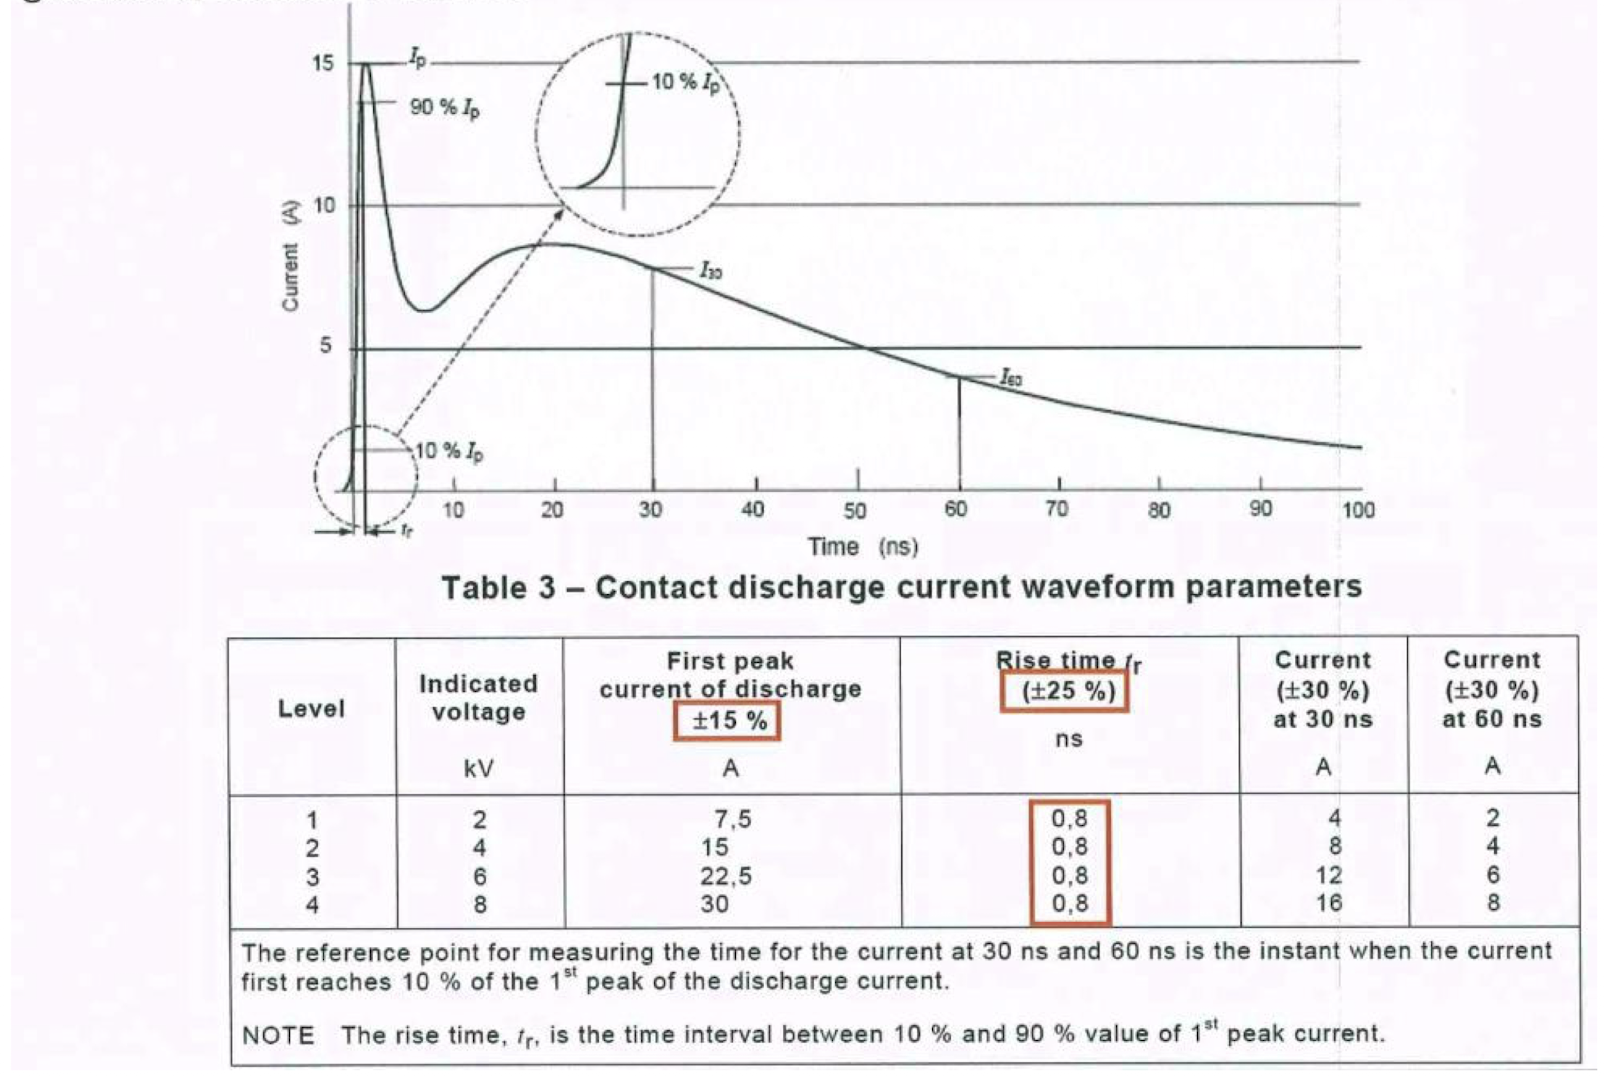
\includegraphics[height=8cm]{src/assets/pictures/lv4_esd_impuls.png}
  \caption{ESD Entladung eines Prüfimpuls gemäß \textit{EN 61000-4-2:2009}}\label{fig:lv4:esd_impuls}
\end{figure}

\subsection{Welche Anstiegszeit und welche Halbwertszeit hat ein ESD Puls?}
Sehr schnelle Anstiegszeiten Subnanobereich. Halbwertszeit \(\approx 30ns\). (Siehe Abbildung~\ref{fig:lv4:esd_impuls})
Anstiegs: 0,5-20ns

\subsection{Wie kann ein ESD Puls in elektronische Schaltungen einkoppeln?}
\begin{itemize}
  \item Galvanisch durch Funkenüberschlag
  \item Induktiv durch \(\frac{di}{dt}\) auf geerdete Teile
  \item Kapazitiv durch \(\frac{du}{dt}\) auf isolierte metallische Teile
  \item Abstrahlung Magnetfeld durch große \(\frac{di}{dt}\)
\end{itemize}

\subsection{Was versteht man unter einen triboelektrischen Effekt?}
Engl.: Triboelectric Charge. Elektrostatische Aufladung durch Berührung/Reibung (Siehe Frage~\ref{sec:lv4:electrostatic}). Verschiebung von Elektronen auf der Metalloberfläche meist durch Berührung und anschließender Trennung => Ladungstransfer zwischen Körpern mit verschiedenem Potential.

\subsection{Welche Maßnahmen werden zum Schutz von elektrostatischer Entladung gesetzt?}
Abhilfe: ESD-Schutzelemente
\begin{itemize}
  \item Elektrostatisch schützende Bodenbeläge
  \item ESD-geeignete Sitzgelegenheiten
  \item Vermeidung unnötiger Isolatoren beispielsweise Kaffeetassen, Klebebänder, Styropor und Kunststofffolien
  \item Verwendung von Ionisatoren zum gezielten Abbau von elektrostatischer Ladung im Produktionsprozess
\end{itemize}

\begin{itemize}
  \item ESD Schutzbeschaltung TVS-Dioden
\end{itemize}

\subsection{Was ist der Unterschied zwischen dem HBM und dem MM?}
HBM, MM und CDM sind verschiedene Aufbauten für ESD Prüfungen.\p
%
\textbf{Human-Body Model (HBM)}\\
Simulation eines ESD durch die Entladung eines Menschen.\p
%
\textbf{Machine Model (MM)}\\
Hier wird das Entladen eines beliebigen Objekts auf das Gerät simuliert.\p
%
\textbf{Charged Device Model (CDM)}\\
Das CDM simuliert die Entladung des statisch geladenen Geräts, wenn es mit einem leitenden Material in Berührung kommt.\p

\subsection{Was ist der Unterschied zwischen Kontakt und Luftentladung? Wann wird welche Entladeart angewandt?}
\textbf{Kontaktentladung:}
Entladung durch Berührung des Geräts oder der Koppelplatte
%
\begin{itemize}
  \item gezielt
  \item reproduzierbar
  \item direkt/indirekt
\end{itemize}
%
\textbf{Luftentladung:}
Entladung über die Luft
%
\begin{itemize}
  \item ungezielt
  \item schlecht reproduzierbar
\end{itemize}

\subsection{Von welchen Einflüssen ist die Reproduzierbarkeit der ESD Luftentladung abhängig?}
\begin{itemize}
  \item Ladespannung
  \item Annäherungsgeschwindigkeit
  \item Umgebungsdruck
  \item Luftfeuchtigkeit
\end{itemize}

\subsection{Wie schaut ein ESD Prüfaufbau aus?}
\begin{figure}[!ht]
  \centering
  \includegraphics[height=8cm]{src/assets/pictures/lv4_prüfaufbau.png}
  \caption{ESD Prüfaufbau}\label{fig:lv4:esd_test}
\end{figure}

\subsection{Wann und warum entstehen Burststörungen?}
Burststörungen sind leitungsgeführte Störungen und treten bei schnellen Schaltflanken auf.

\subsection{Welches Frequenzspektrum hat ein Burstpuls?}
Unterschiedliche Bandbreiten möglich. Bandbreite steigt je kürzer der Impuls ist.\\
siehe Abbildung \ref{fig:lv4:electro_interferences}
\begin{figure}[ht]
  \centering
  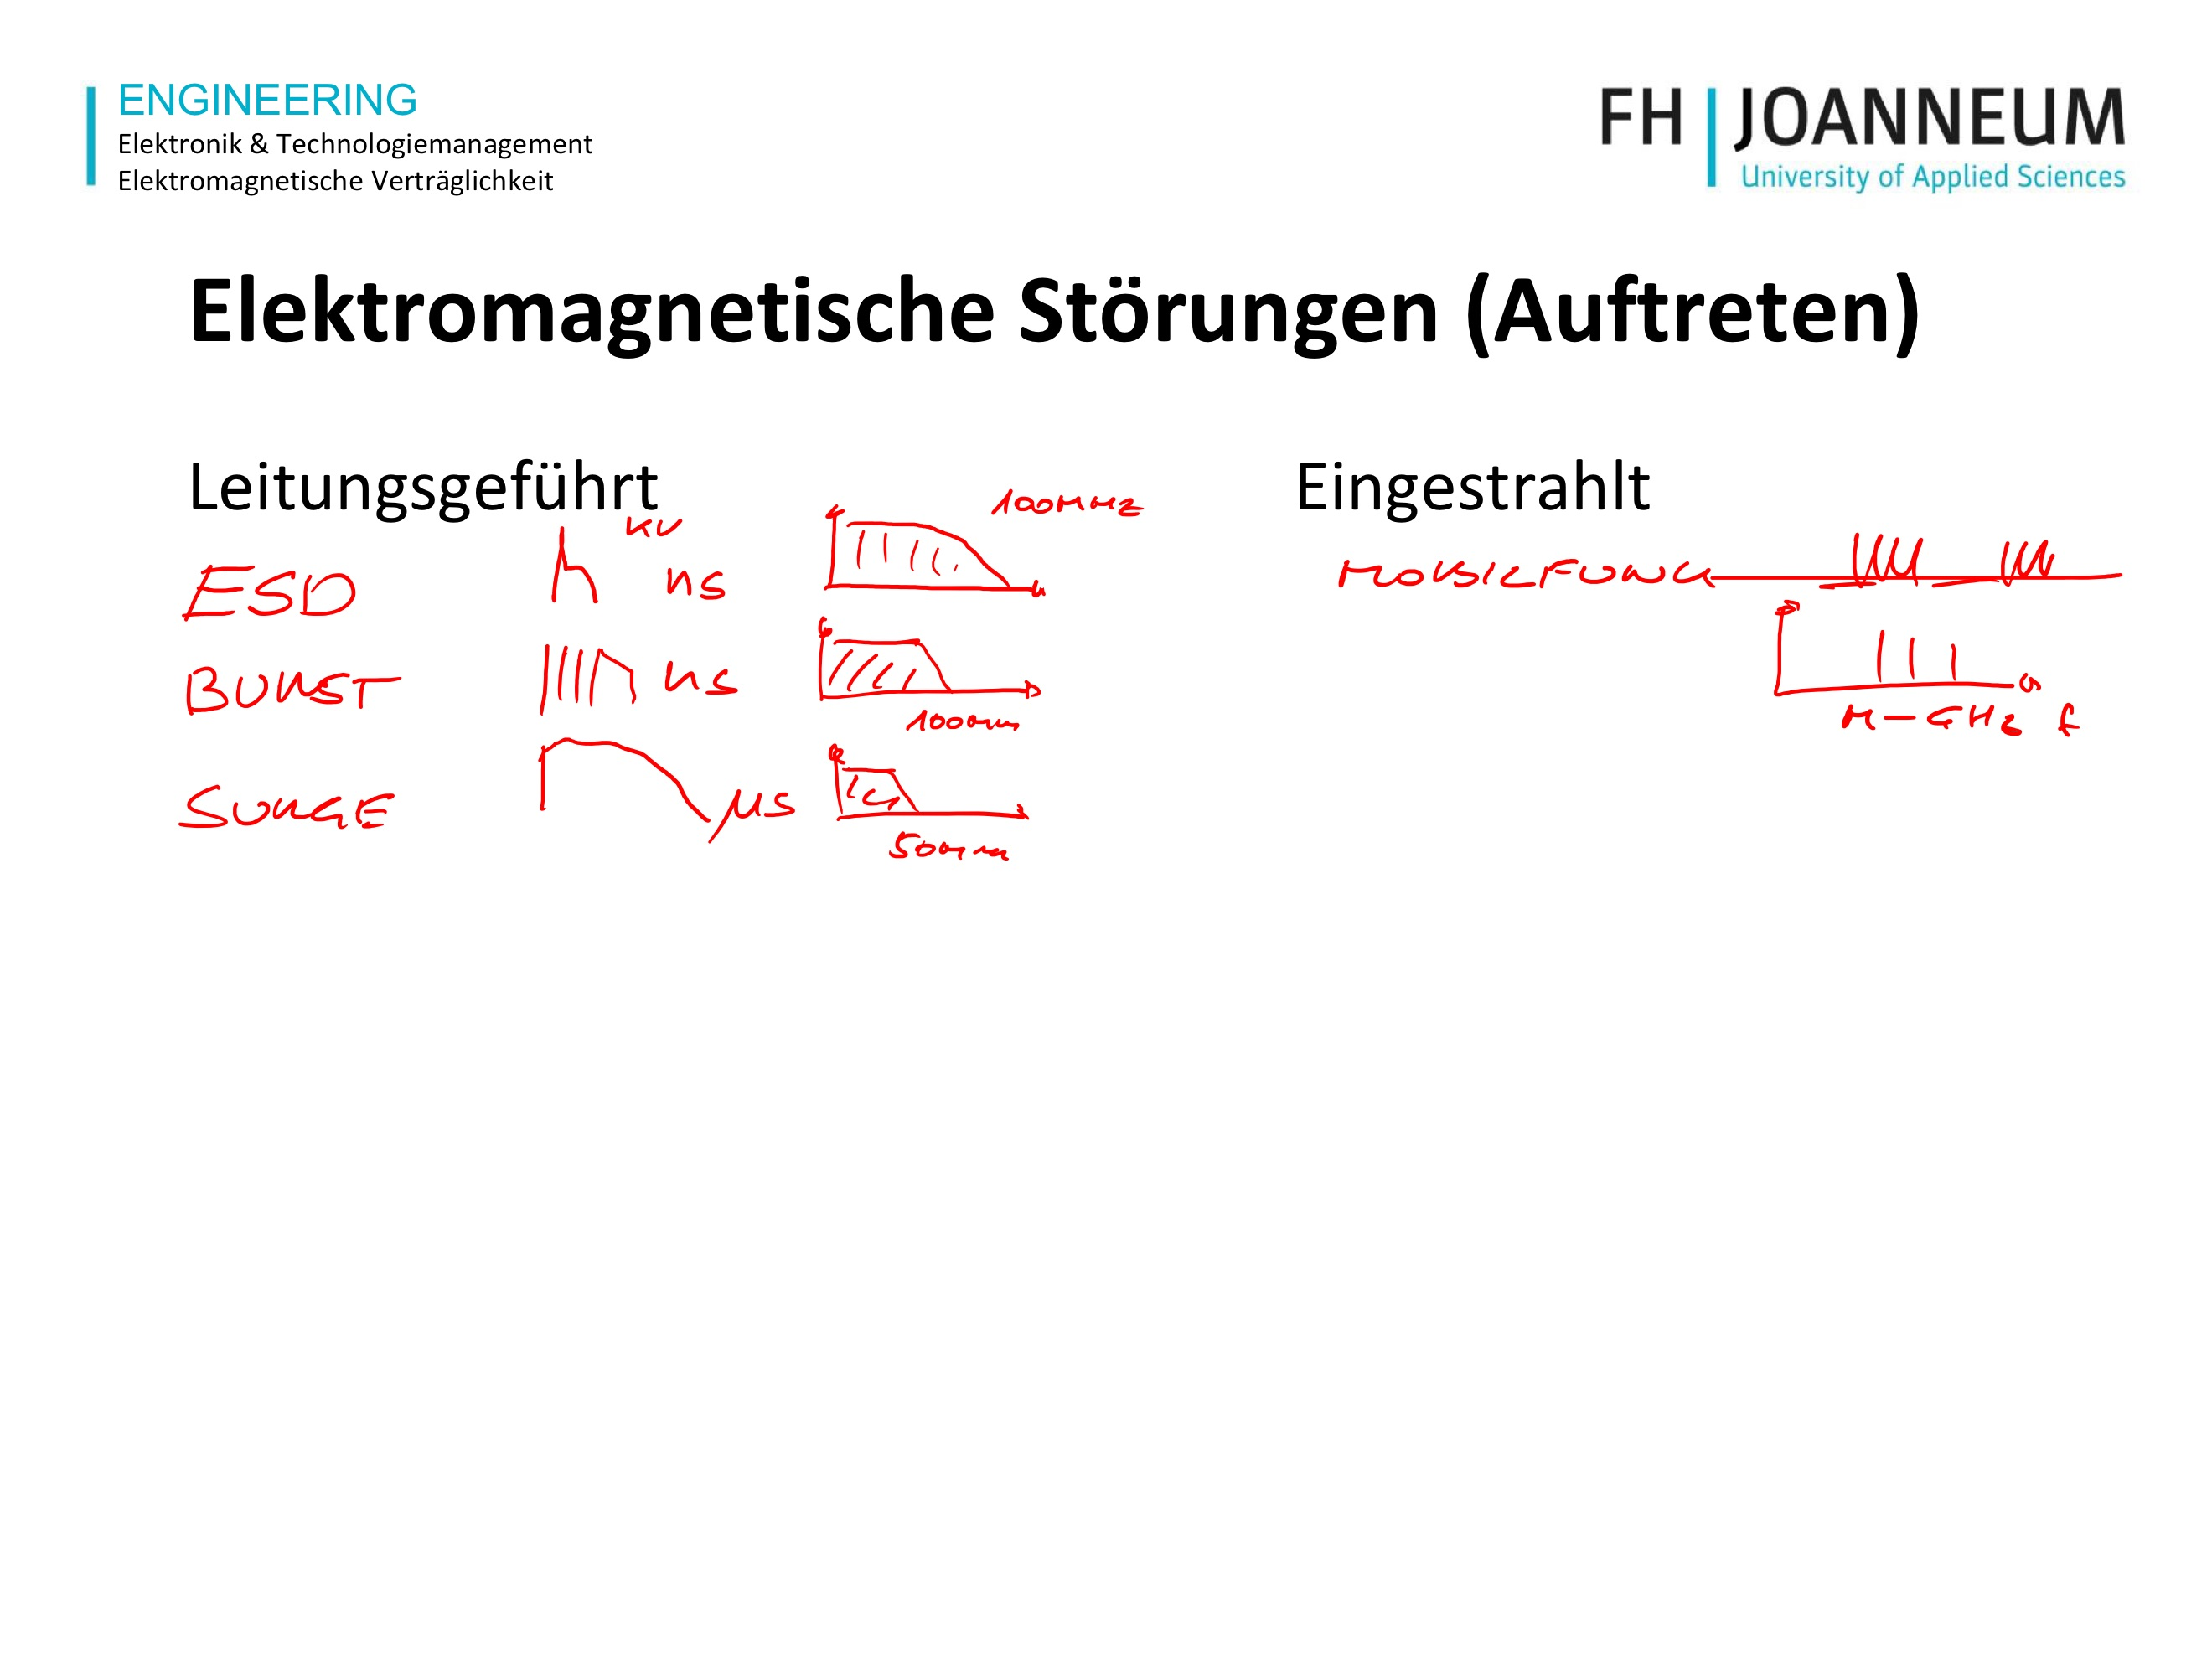
\includegraphics[height=7cm]{src/assets/pictures/lv4_elektromagnetische_stoerungen.jpg}
  \caption{Elektromagnetische Störungen, Auftreten und Frequenzspektrum}\label{fig:lv4:electro_interferences}
\end{figure}

\subsection{Mit welchen Spannungs- und Stromhöhen ist beim Burststörungen zu rechnen?}

\subsection{Welche Anstiegszeit und welche Halbwertszeit hat ein Burstpuls?}
Anstiegszeit \(\approx 5ns \pm 30\%\). Halbwertszeit \(\approx 50ns \pm 30\%\). (Siehe Abbildung~\ref{fig:lv4:burst_impuls})

\begin{figure}
  \centering
  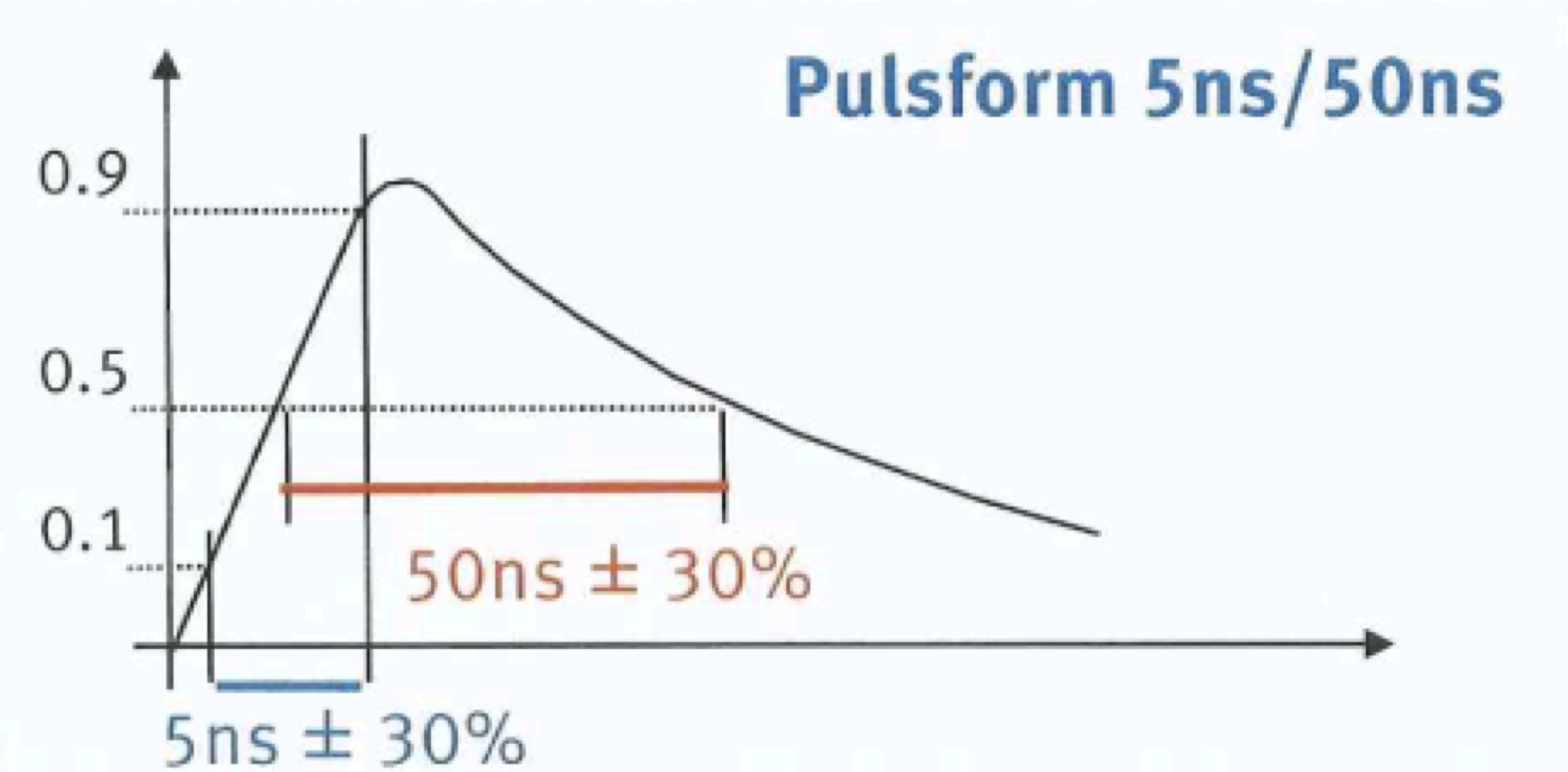
\includegraphics[height=5cm]{src/assets/pictures/lv4_burst_impuls.png}
  \caption{Burst Prüfimpuls}\label{fig:lv4:burst_impuls}
\end{figure}

\subsection{Wie viele Pulse hat ein Burstpaket?}
Ein Burstpaket entsteht beispielsweise aufgrund der Prellwirkung eines Schalters. Es entstehen somit mehrere aufeinanderfolgende Burstpulse.\p
Für die Burstprüfung wird alle \(300ms\) ein \(15ms\) langes Burstpaket ausgelöst. Ein Brustpaket hat \(6\) Pulse

\subsection{Welche Einkopplungsmöglichkeiten kennt man bei der Burstprüfung?}

\subsection{Wie können Burststörungen in elektronischen Schaltungen reduziert werden?}

\subsection{Wann und warum entstehen Surgestörungen?}
Surgestörungen sind leitungsgeführte Störungen und treten bei Überspannungen durch einen Blitzeinschläge auf.

\subsection{Welches Frequenzspektrum hat ein Surgepuls?}
siehe Abbildung \ref{fig:lv4:surge_puls}
\begin{figure}[ht]
  \centering
  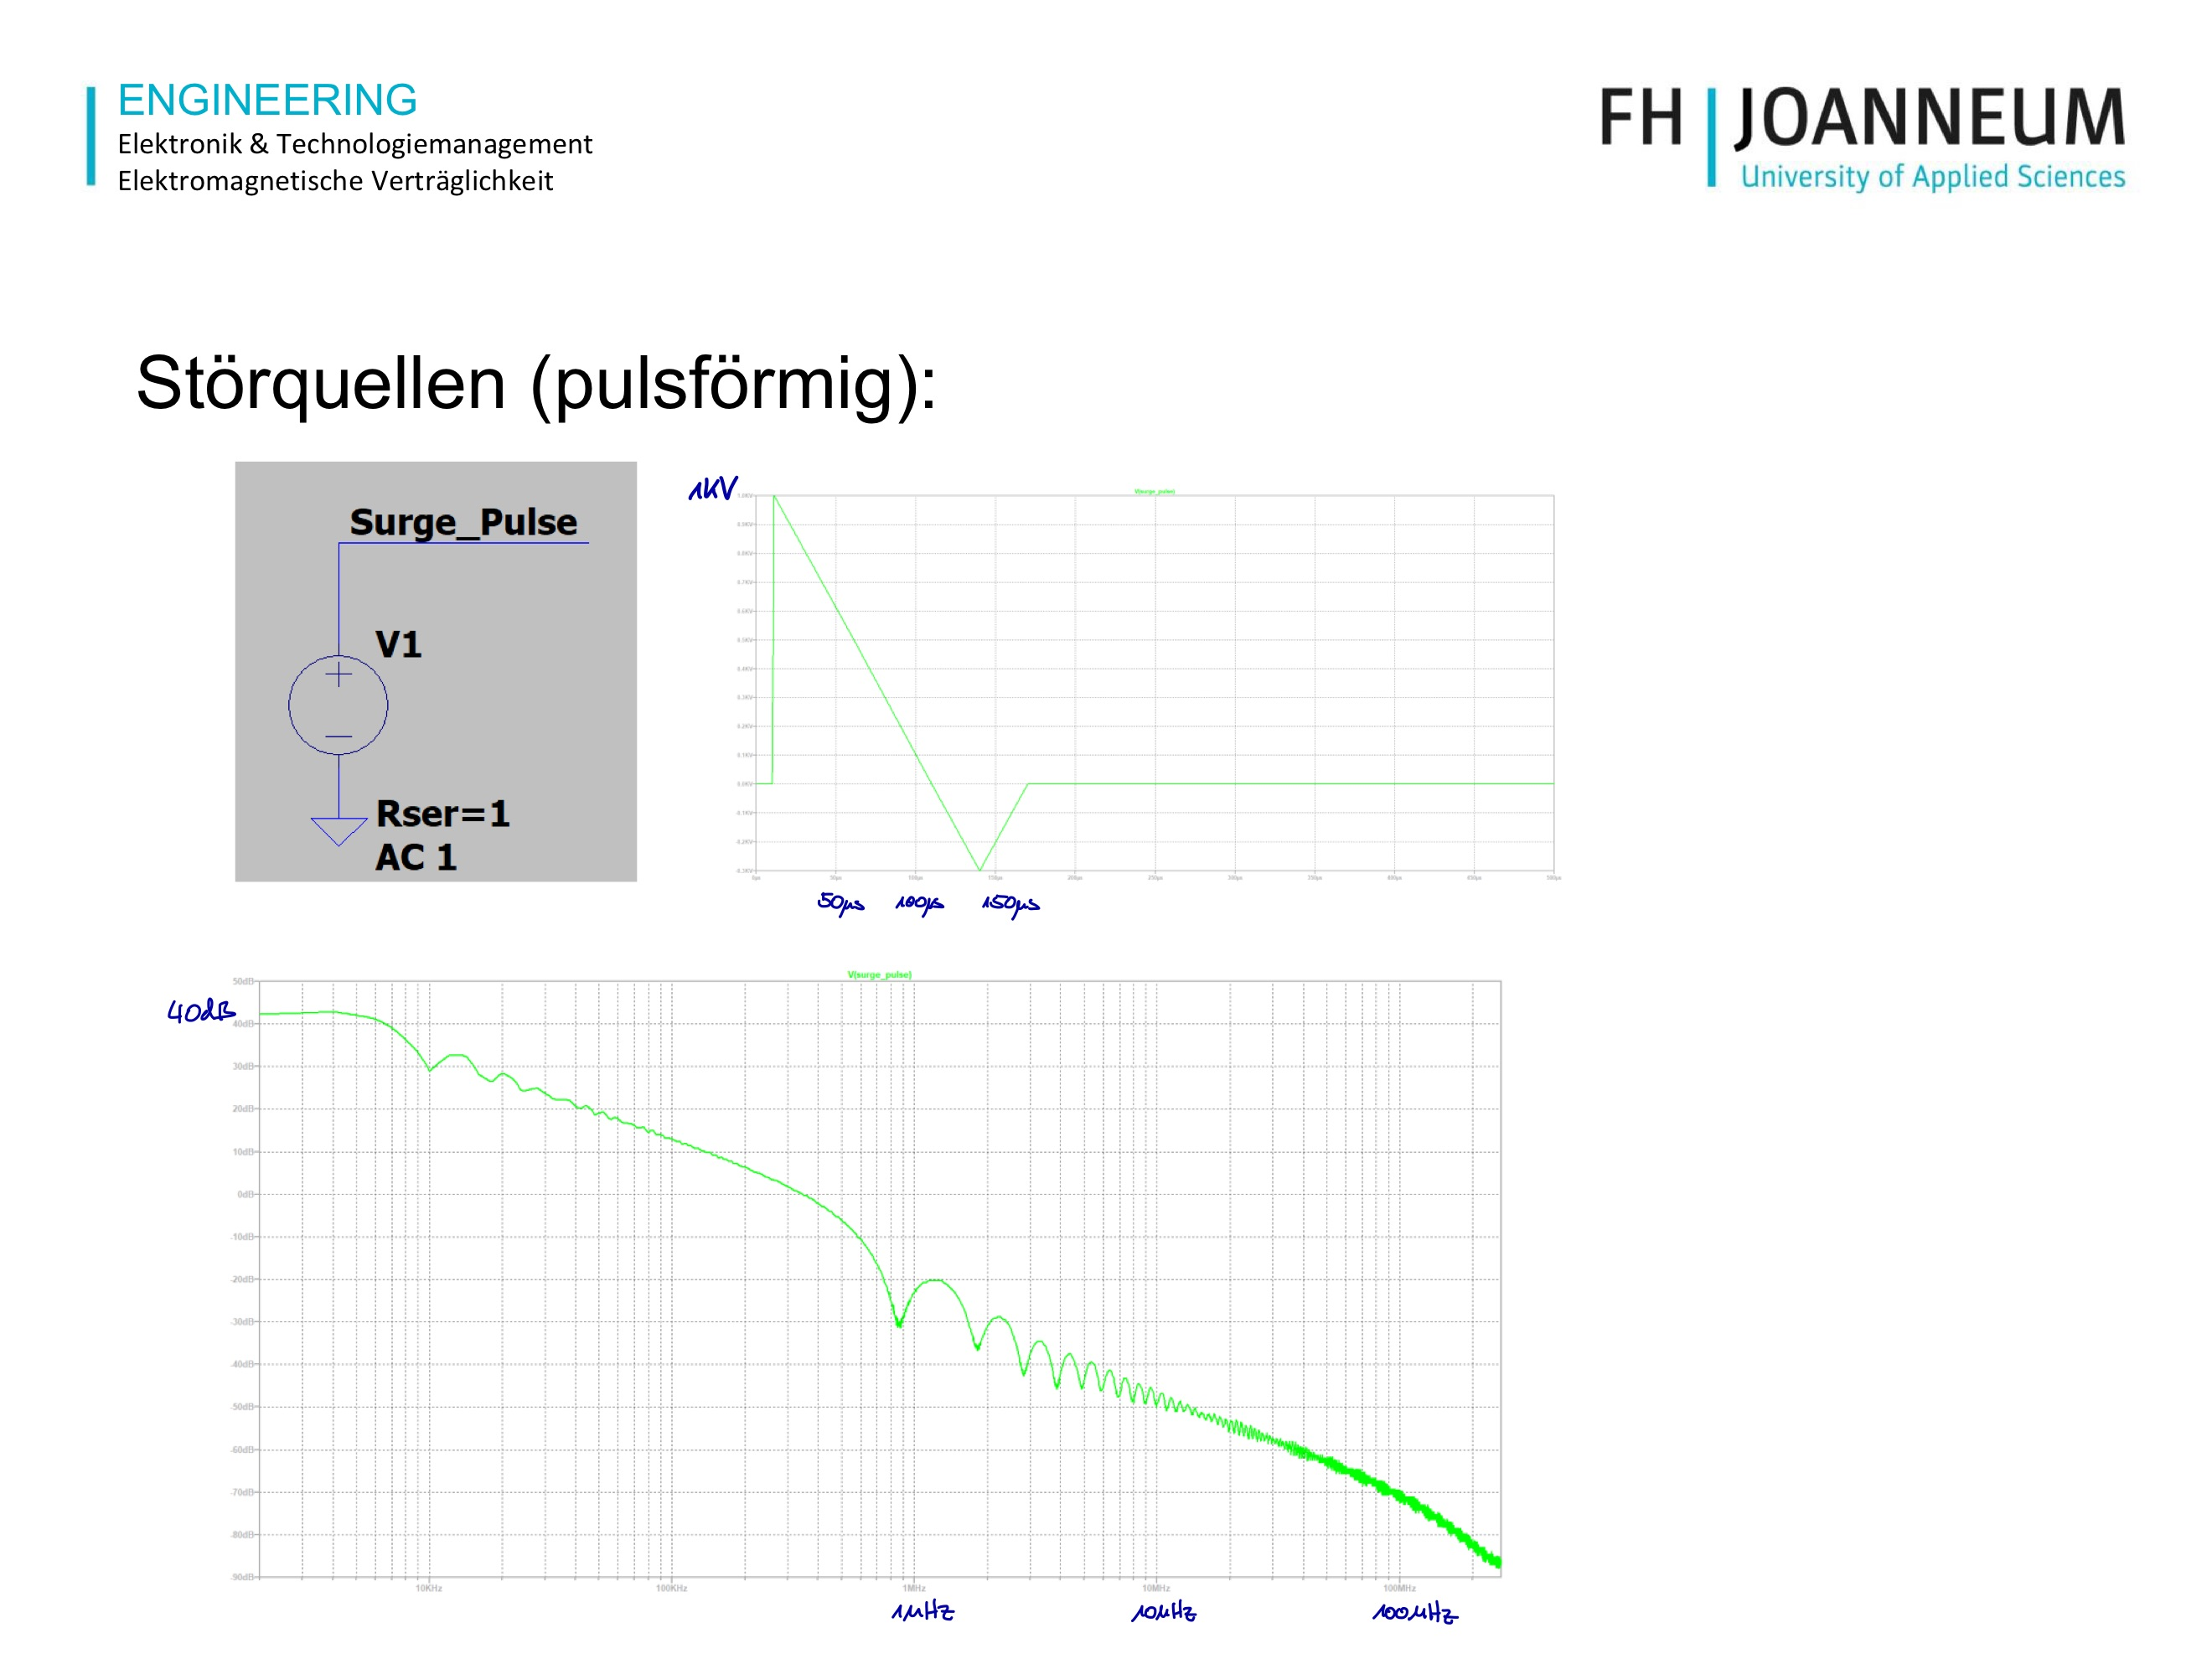
\includegraphics[height=7cm]{src/assets/pictures/lv4_surge_pulse.jpg}
  \caption{Elektromagnetische Störungen, Auftreten und Frequenzspektrum}\label{fig:lv4:surge_puls}
\end{figure}

\subsection{Mit welchen Spannungs- und Stromhöhen ist beim Surge zu rechnen?}
Spannungen bis in den KV-Bereich

\subsection{Wie können elektronische Schaltungen vor Surge geschützt werden?}


\subsection{Auf welchen Leitungen werden Surge- und Burststörungen üblicherweise eingekoppelt?}

\pagebreak
